\documentclass[prb,preprint]{revtex4-1} 

\usepackage{amsmath}  
\usepackage{amsfonts} 
\usepackage{graphicx} 

\begin{document}


\title{Franck-Hertz Experiment; Measuring Energy Levels of Neon and Mercury}

\author{Jiajun}
\email{XXX} 
\affiliation{XXX}


\author{Danika Luntz-Martin}
\email{dluntzma@smith.edu}
\affiliation{Department of Physics, Smith College, Northampton, MA , 01063}


\date{\today}

\begin{abstract}


\end{abstract}


\maketitle 


\section{Introduction} 


\section{Methods}

\subsection{Neon}
\subsection{Mercury}


\section{Results}

\subsection{Neon}

We did four data runs using neon. For each run we recorded the accelerating voltage (x data) and the electron current measured by the anode???, this current was recorded as a voltage measured across an internal resister. Each of our runs showed three discernible dips in the voltage corresponding to electron current, see the sample data run Figure~\ref{neon_data}. These dips are the voltages just before the electrons have enough energy (from the accelerating voltage) to reach the anode even after an inelastic collision with a neon atom. The apparent double minima, see the second and third dips in Figure~\ref{neon_data}, is most likely caused by by energy levels with very similar excitation energies.~\cite{XXX} Also of interest is the voltage corresponding to the steepest negative slope which is when the majority of electrons have enough energy to cite the neon atoms. However the location of the steepest negative slope was difficult to determine from our data, again see Figure~\ref{neon_data}.

\begin{figure}[h!]
\centering

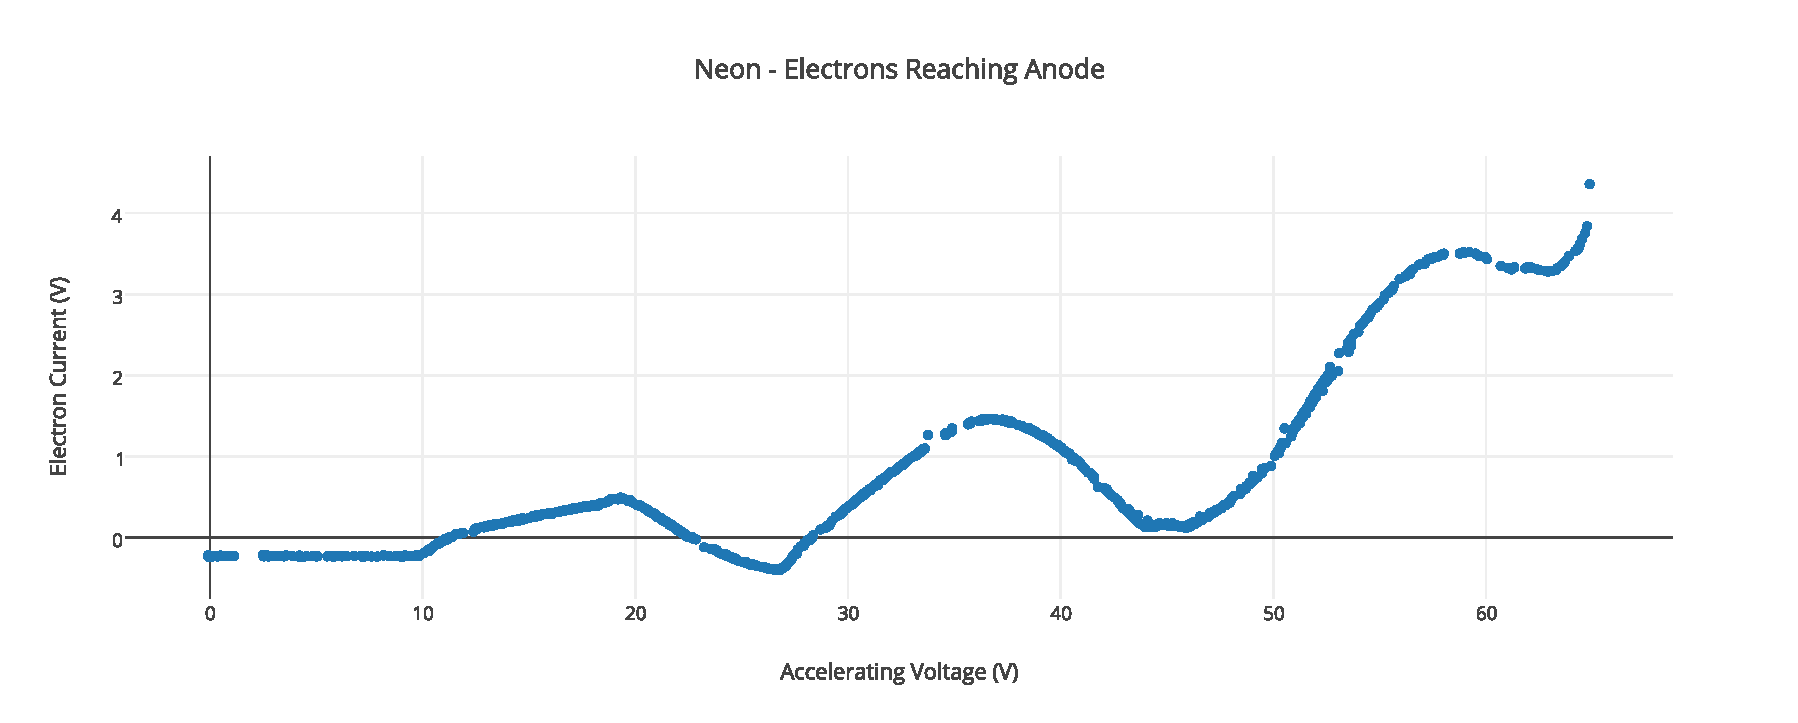
\includegraphics[width=6in]{neon_data.pdf}
\caption{Neon data with electron current as a voltage plotted against accelerating voltage. The three dips correspond to electrons exciting three neon atoms before reaching the anode. The double minima in the second and third dips is due to multiple excitations with similar energies.}

\label{neon_data}
\end{figure}


\subsection{Mercury}

Since the number of discernible dips for mercury depends on temperature, we collected data for 10$^{\circ}$ C increments starting at 150$^{\circ}$ C and ranging to 210$^{\circ}$ C. From this data, see Figure~\ref{hg_data}, it can be seen that there is an optimum temperature at around 200$^{\circ}$ C at which the most dips can be observed. 

\begin{figure}[h!]
\centering

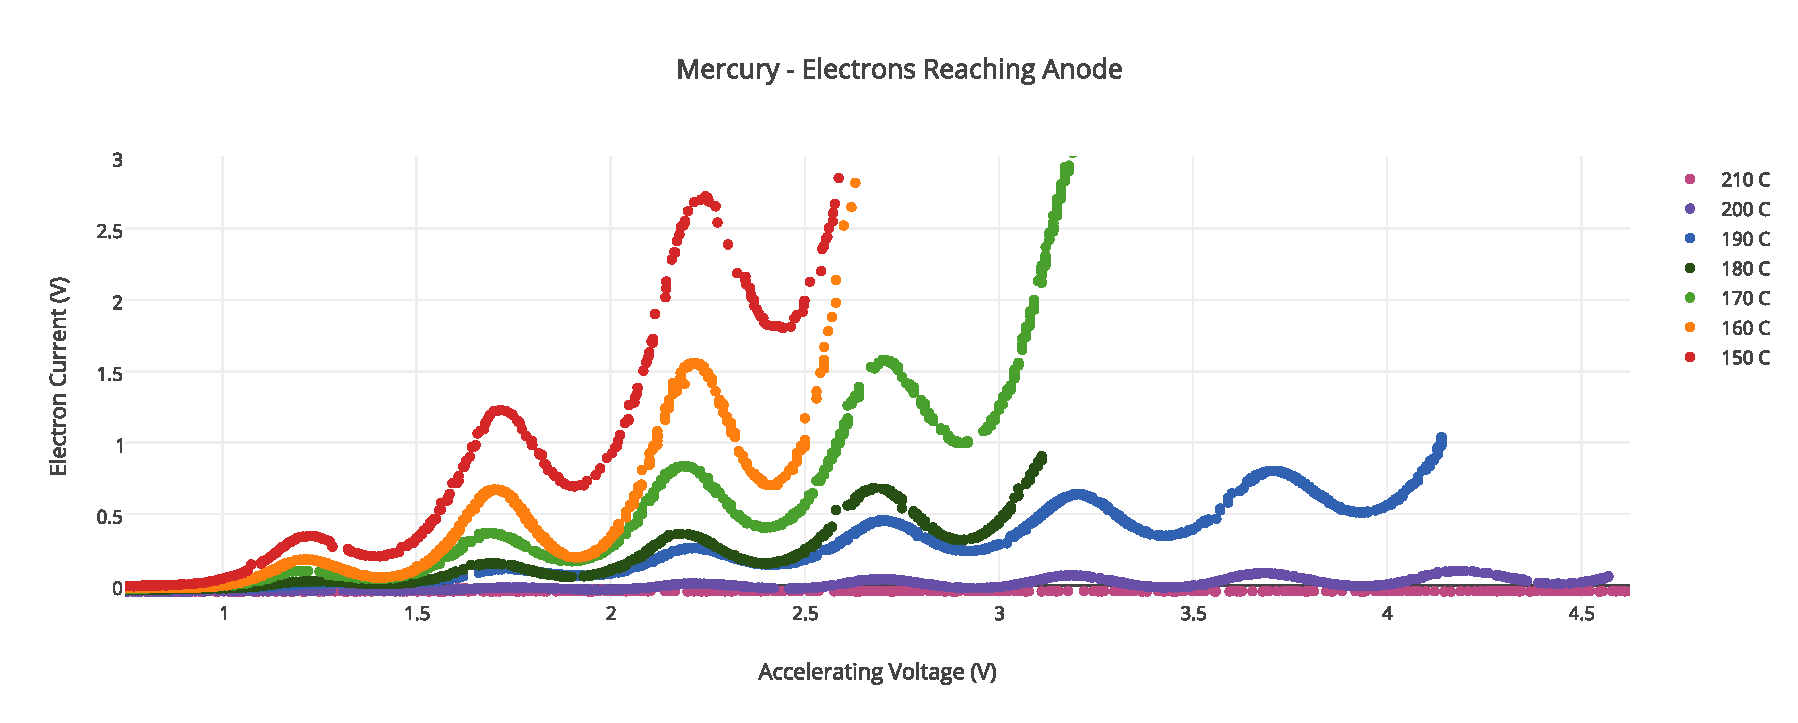
\includegraphics[width=6in]{hg_data.pdf}
\caption{Mercury data for temperatures ranging from 150$^{\circ}$ C to 210$^{\circ}$ C. The range of temperatures shows the optimum temperature to be approximately 190 - 200$^{\circ}$ C. For higher temperatures, such as 210$^{\circ}$ C, the dips in electron current are not discernible. For lower temperatures, for example 150$^{\circ}$ C and 160$^{\circ}$ C, there were fewer dips before the mercury atoms ionized.}

\label{hg_data}
\end{figure}

Using the information that we obtained about the optimum range of temperature, we took a more data using a lock-in. With the lock-in we took data from 185$^{\circ}$ C to 215$^{\circ}$ C in increments of 5$^{\circ}$ C. The output from the lock-in, see Figure~\ref{hg_lockin}, is the derivative of the output without the lock-in. Therefore, the dips in the lock-in output correspond to the steepest negative slope of the direct output and the places the lock-in data passes through zero correspond to the dips and peaks of the direct output.

\begin{figure}[h!]
\centering

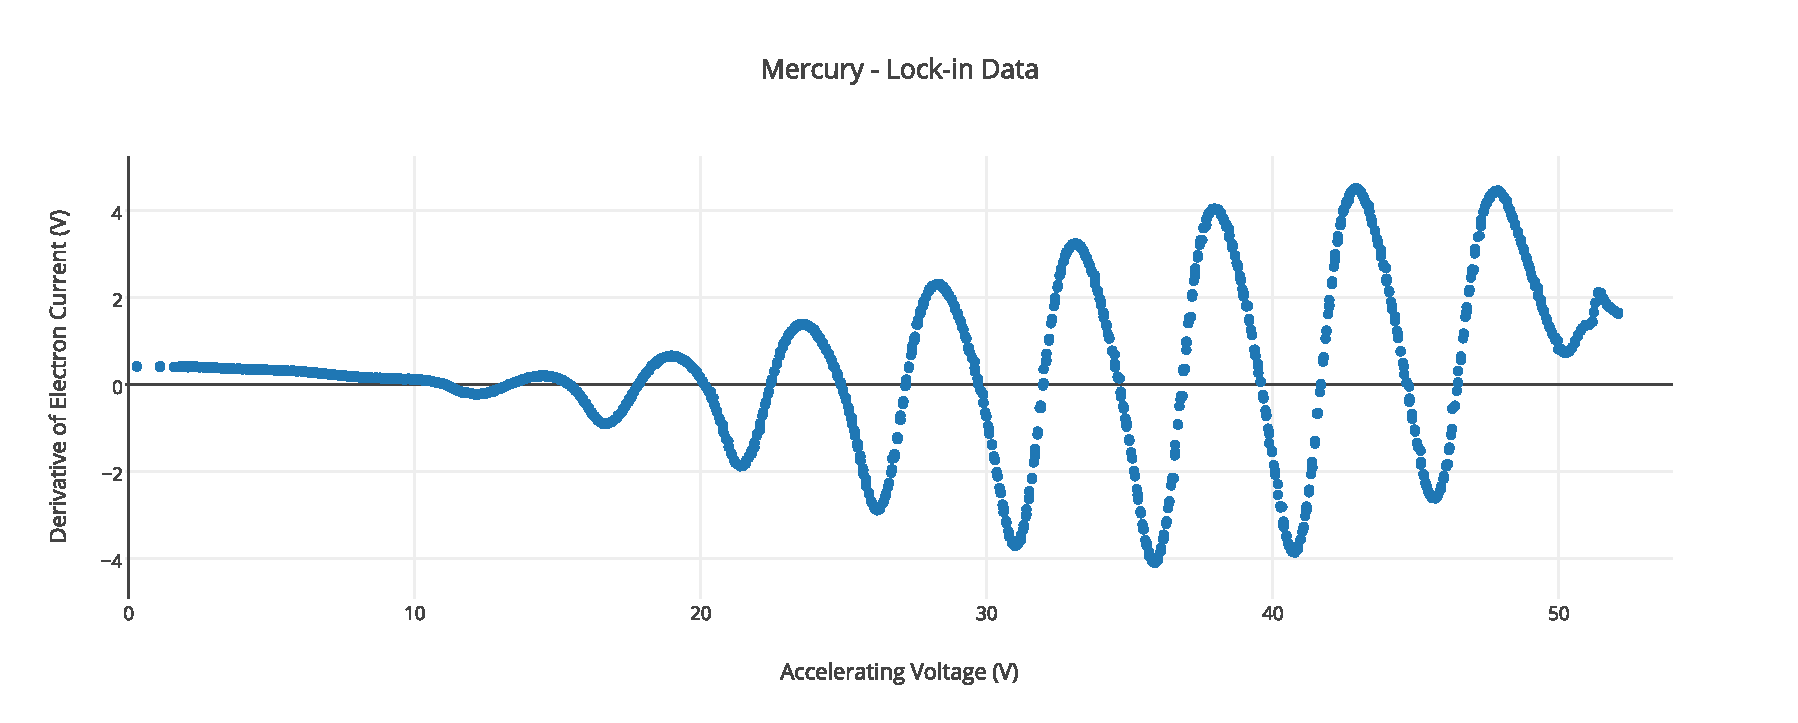
\includegraphics[width=6in]{hg_lockin.pdf}
\caption{}

\label{hg_lockin}
\end{figure}



\section{Analysis}

\subsection{Neon}
\subsection{Mercury}

\section{Discussion}


\section{Conclusion}



\begin{thebibliography}{9}


\bibitem{latexsite} \LaTeX\ Project Web Site, \url{<http://www.latex-project.org/>}.

\bibitem{latexbook}Helmut Kopka and Patrick W. Daly, \textit{A Guide to
\LaTeX}, 4th edition (Addison-Wesley, Boston, 2004).

\bibitem{revtex} REV\TeX\ 4 Home Page, \url{<https://authors.aps.org/revtex4/>}.

\bibitem{cloudLaTeX} On the other hand, you can avoid the installation process
entirely by using a cloud-based \LaTeX\ processor such as ShareLaTeX,
\url{<https://www.sharelatex.com/>}, or write\LaTeX, \url{<https://www.writelatex.com/>}.

\bibitem{mermin} N. David Mermin, ``What's wrong with these equations?,'' 
Phys. Today \textbf{42} (10), 9--11 (1989).  
% Note that the issue number (10) in this citation is required, because
% each issue of Physics Today starts over with page 1.  Also note the use of
% an en-dash (--), not a hyphen (-), for the page range.

\bibitem{feynman} Richard P. Feynman, Robert B. Leighton, and Matthew Sands, 
\textit{The Feynman Lectures on Physics, Vol.\ 1} (Addison-Wesley, 1964), p.~3-10.
% Note that this book is paginated by chapter; "3-10" is a single page reference
% that uses a hyphen, not a range of pages that would us an en-dash (--).


\end{thebibliography}


\end{document}
